\clearpage
\fancyhead[R]{\sffamily\small\color{Muted}Vulkan / 显存与光照}
\section{Sponza 的光照数据放在哪里}

在原生分辨率下观察 Sponza 中庭，显卡需要为每个像素找出射线碰到的墙面，读取材质，再结合前几帧的结果计算光照。这会反复读取三角形、用来查找三角形的包围盒树，以及保存历史颜色的数组。旧版为了让 CPU 可以直接填数组，选择了第一个允许 CPU 读写的 Vulkan 内存类型。这台笔记本上的第一个匹配项是系统内存。着色器虽然在独立显卡上运行，读取大数组时却要经过连接显卡与主机的 PCIe 总线。

本机是 NVIDIA GeForce RTX 5070 Ti Laptop GPU，驱动 616.56。驱动报告了 11.66\,GiB 的显卡本地内存和 15.90\,GiB 的系统内存。原规则选中类型 2，属于系统内存。类型 4 同时允许显卡本地读取和 CPU 映射，使用的是同一份 11.66\,GiB 的本地内存。把计算数组放到类型 4 后，加载器仍然可以把初始数据写进去。随后显卡每帧读取三角形和反复更新历史颜色时，主要使用自己的显存。

\subsection{用同一个编辑器画面比较}

两个 Debug 编辑器从相同的对象文件和引擎库链接，试验版本只替换计算数组选择的内存。打开同一份 \code{Sponza-Atrium.redflag}，固定机位，场景面板为 $1442\times964$ 像素。使用 Lit、Native、全点光源、DDGI、GTAO 和 TAA，DDGI 采样数为 2，SSR 关闭。两组都启用 Vulkan 验证层，采用同样的显示设置。打开场景后的首次模型导入与初始化不计时。每次运行再去掉 4 次预热的光照累积，统计接下来的 21 次。测量发生在静止图像停止刷新之前。

\begin{center}\smalltable
\begin{tabular}{lrrrr}
\toprule
运行次序 & 第 1 轮 & 第 2 轮 & 第 3 轮 & 第 4 轮\\
\midrule
计算数组所在位置 & 系统内存 & 本地显存 & 本地显存 & 系统内存\\
光照累积中位数（毫秒） & \memoryRunTimes\\
\bottomrule
\end{tabular}
\end{center}

把相同配置的两轮合并，各有 42 个样本。光照累积耗时的中位数从 \memoryOld\,ms 降至 \memoryNew\,ms。这个时间从 CPU 开始更新光照，到所有同步提交的 GPU 工作完成，倍率约为 $\memoryRatio$。它覆盖光照调度与等待。编辑器界面、图像呈现和其余渲染工作另行计时，因此不能把上述时间直接换算成编辑器帧率。

\clearpage
\subsection{回放同一张图，核对显卡的耗时}

为了检查显卡的工作本身有没有减少等待，用相同的 Stanford Bunny 场景各截一帧。在 $288\times192$ 下，两份 RenderDoc 帧里都有 12 次计算调度。先回放一次预热，再用 GPU 时间计数器采样 7 次，表中列出三道计算的中位数。探针更新需要查找射线打中的三角形；GTAO 则反复读取附近像素的可见表面，两者都要多次访问显存中的数组。

\begin{center}\smalltable
\begin{tabular}{lrrr}
\toprule
计算内容 & 事件编号 & 系统内存（毫秒） & 本地显存（毫秒）\\
\midrule
\memoryGpuRows
\bottomrule
\end{tabular}
\end{center}

回放脚本定位两份帧里相应事件的输出数组。DDGI、ReSTIR GI、ReSTIR DI、直接光、GTAO、屏幕反射、分簇点光和 TAA 共八张结果，每张都是四通道浮点图；逐字节对照全部一致。两份帧都没有调试消息。这组 GPU 时间只描述兔子场景的单道计算，前页的 Sponza 数据来自实际运行的编辑器。

\subsection{其他显卡怎样上传和读回}

实现位于 \code{VulkanComputeDevice::CreateBuffer}。先选择适合计算的本地显存；在最大的兼容显存堆上，优先选 CPU 能直接映射、写后双方可见的类型。只有小块显存能映射时，大数组保留在容量更大的主显存中。上传先把三角形写入暂存缓冲区，再让 GPU 复制到本地数组。读回时则由 GPU 把结果写入暂存缓冲区，待复制完成后交给 CPU。用独立测试构建强制选择本机不可映射的类型 1，三帧、35 个数组元素与 $7\times5$ 历史图均通过逐项核验。该测试检查的是这条上传和读回路径，其他型号显卡上的速度仍待实测。

\noindent\small\color{Muted}
原始 Chrome 时间线、驱动内存类型、逐帧毫秒值和 RenderDoc 回放记录位于
\path{output/profiling/compute-memory/}。对照脚本为 \path{tests/profile_compute_memory.py}。
暂存复制的接口可对照 \href{https://docs.vulkan.org/refpages/latest/refpages/source/vkCmdCopyBuffer.html}{Khronos 的 vkCmdCopyBuffer 说明}。\normalsize\color{Ink}

\clearpage
\subsection{移动相机与停手后的整帧时间}

这组历史记录测的是显存分配调整前后的编辑器，当时快速导航会切到材质底色。打开 Sponza，把场景面板调到 $948\times613$ 像素，先保持镜头不动，等面板开始沿用最后一张图。然后每隔 150\,ms 滚动一次鼠标滚轮，连续五次拉近、五次拉远，共 50 次。下表以毫秒统计完整一帧从开始到结束经过的时间，其中包含 UI、GPU 等待以及呈现。P95 表示约有 95\% 的帧在这个时间内完成。

\begin{center}\smalltable
\begin{tabular}{lrrrr}
\toprule
画面 & 旧版中位数 & 新版中位数 & 新版 P95 & 新版帧数\\
\midrule
\memoryNavigationRows
\bottomrule
\end{tabular}
\end{center}

第一行关闭“快速移动相机”。变焦过程中，显卡持续计算直接光、DDGI、GTAO 和 TAA，滚动触发的 50 个相机运动帧均进入统计。旧版同一输入只有 25 个帧观察到单独的运动，耗时较长时会在两次绘制之间收到多次滚动。第二行启用“快速移动相机”，移动过程中显示相同尺寸的材质底色图。停手后恢复完整光照并逐帧累积，缓存稳定后进入第三行。时间相近的后两行对应两种可见画面。

\begin{figure}[H]\centering
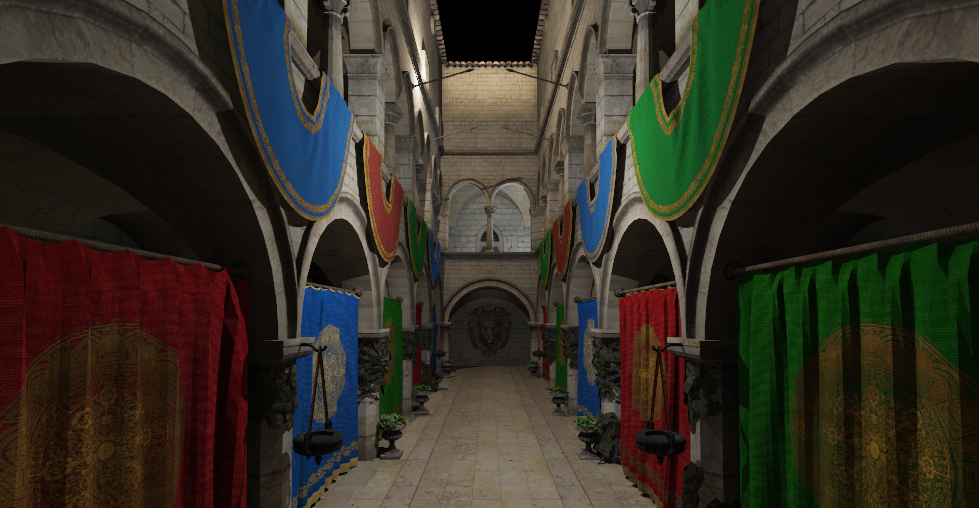
\includegraphics[width=.70\linewidth]{../editor-guide/figures/atrium.png}
\caption{正式 Vulkan 编辑器中的 Sponza 中庭，取自《编辑器使用手册》的实际视口。滚轮既改变栏杆在图上的位置，也改变为光照查找可见表面的视线。}
\end{figure}

该表用于比较新旧编辑器的整帧表现。前面只改内存分配的四轮对照则单独测量了存储数组位置的影响。同一测量目录中的 \code{final-navigation.json} 记录了每项统计，旁边保留两次正式运行的 Chrome 时间线。复现入口为 \path{tests/profile_native_navigation.py}。
